\begin{blocksection}
\textbf{There are three steps to writing a recursive function:}
\begin{enumerate}
    \item Create base case(s)
    \item Reduce your problem to a smaller subproblem and call your function recursively to solve the smaller subproblem(s)
    \item Use the subproblems' solutions as pieces to construct a larger problem's solution (This can happen in many layers!)
\end{enumerate}

\vspace{3mm}

\textbf{Real World Analogy for Recursion}


Imagine that you're in line for boba, but the line is really long, so you want to know what position you're in. 

\begin{center}
	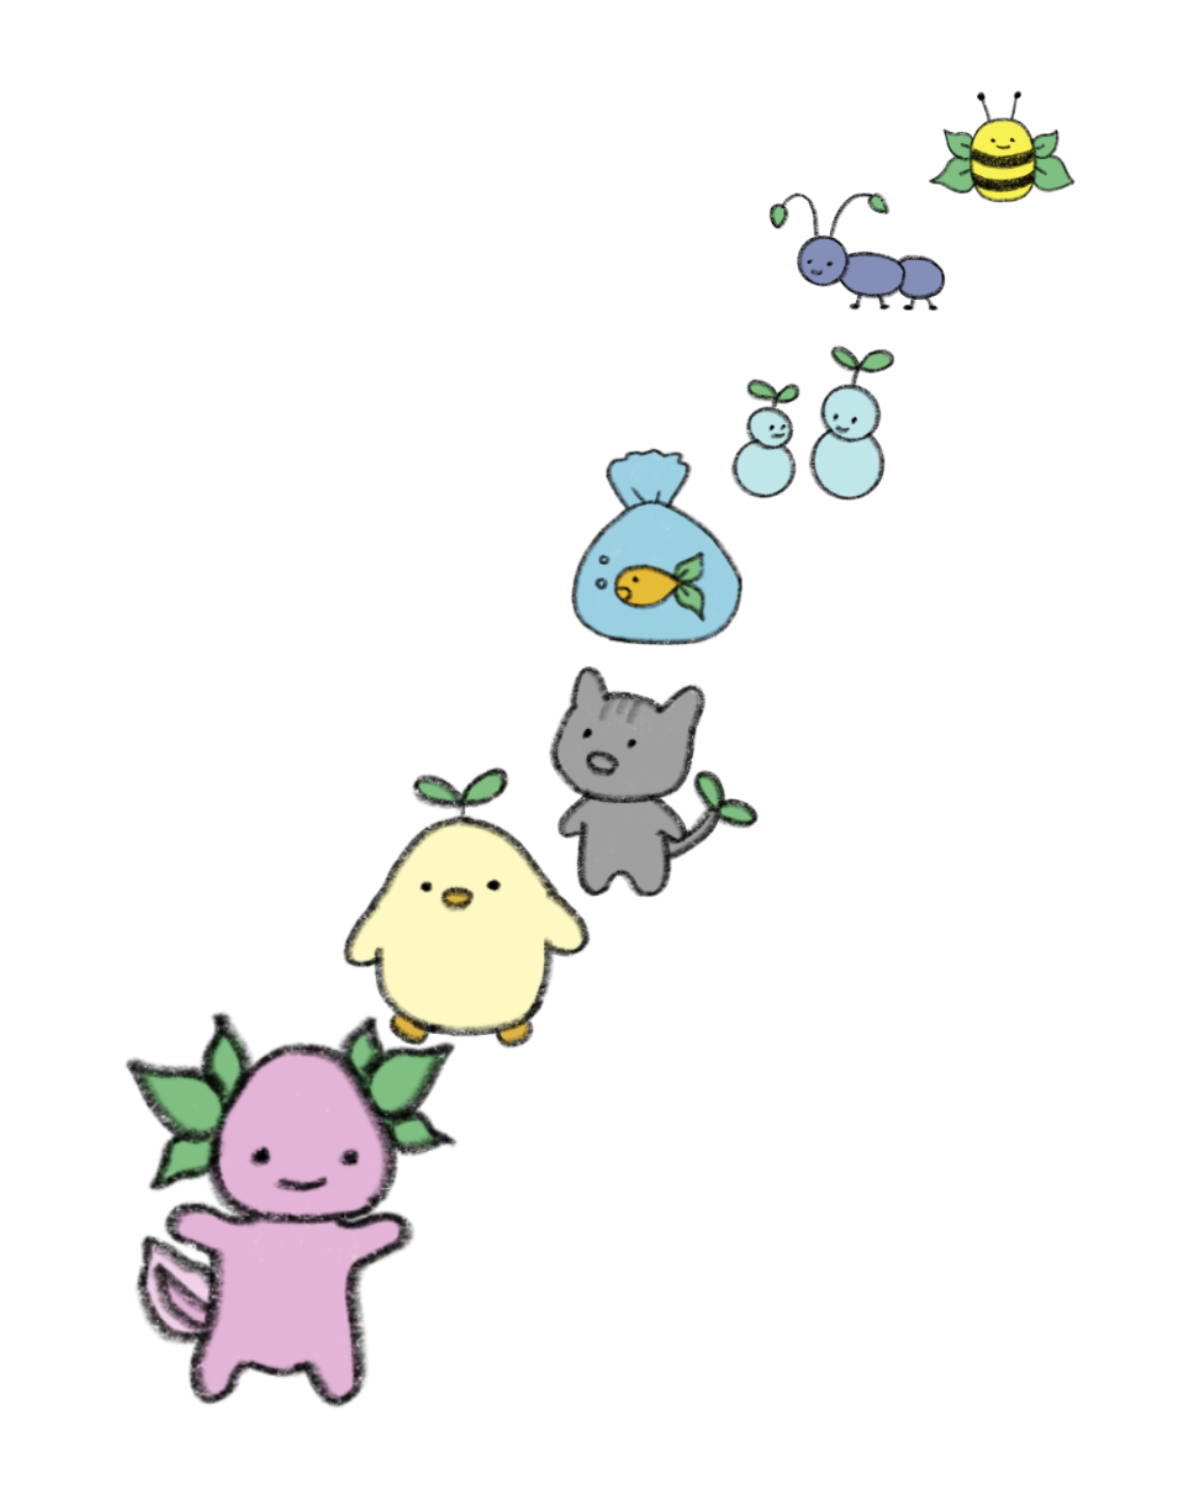
\includegraphics[scale=0.5]{Mascots.PNG}
\end{center}

You decide to ask the person in front of you how many people are in front of them. That way, you can take their response and add 1 to it to find your place. Now, the person in front of you is faced with the same problem that you were trying to solve, with one less person in front of them than you. They decide to take the same approach that you did by asking the person in front of them. This continues until the very first person in line is asked. At this point, the person at the front knows that there are 0 people in front of them, so they can tell the person behind them that there are 0 people in front. Now, the second person can figure out that there is 1 person in front of them, and can relay that back to the person behind them, and so on, until the answer reaches you.

Looking at this example, we see that we have broken down the problem of ``how many people are there in front of me?'' to 1 + ``how many people are there in front of the person in front of me''? This problem will terminate with the person at the front of the line (with 0 people in front of them). Putting this into more formal terms, we are breaking down the problem into a \textbf{recurrence relationship}, and the termination case (when the question gets to the very first person in line) is called the \textbf{base case}.
\end{blocksection}


\begin{blocksection}
As a program goes through recursion, it doesn't formally solve the problem until it reaches the base case, in which case it works its way up from the base case to the original input to construct your final answer. Just like your question as you stand in line, the program: 

\begin{enumerate}
	\item goes out (down the call stack), person by person (call by call) \textbf{(recursive case)}
	\item until the person at the very front is reached \textbf{(base case)}
	\item when the answers get added onto and eventually passed back to you, solving the problem. \textbf{(constructing the final solution with solutions to subparts)}
\end{enumerate}

\end{blocksection}

\begin{meta}
\textbf{Teaching Tips}
\begin{enumerate}
	    \item Base Case - What is the simplest case? Or in what case do you want your recursion to stop? It's helpful to use edge cases to nudge students if they get stuck.
	    \item Break the problem down into smaller problems (Try to address this in terms of each specific problem, then extrapolate for general understanding)
	    \begin{itemize}
			\item What do you need to do to reach your base case?
			\item For example: in factorial (usually seen in lecture), we have to subtract by one each time we do a recursive call
		\end{itemize}
		\item Solve the smaller problem recursively
		\begin{itemize}
			\item How would you use the solution to the smaller problem to write a solution to the original problem?
			\item "Recursive Leap of Faith"---When writing the recursive statement, assume the function works as intended for the smaller problems. Trust. (Abstraction! woohoo!)
			\item If you don't know what the recursive call needs to be, you can take an educated guess and see what happens. 
			\item It's often extremely helpful to run line by line through a doctest to test both a tentative solution and your understanding to a problem.
			\item When running through a problem, it's often helpful to find a way to visualize the recursion in action! For shorter problems, one way you can do this is through drawing a stack of ``boxes,'' each containing the result of a recursive call inside them, going all the way until the base case. Other linear visualizations work also!
		\end{itemize}
\end{enumerate}
We tend to throw around the term ``recursive leap of faith'' a lot, and I think that it confuses students. The ``recursive leap of faith'' is not synonymous with ``the recursive call is correct''. Rather it's a specific assumption we make while writing a recursive function that the recursive calls we make produce the correct output, even if we're not done writing our function. That is, the function we're writing works even if we're not done writing it. The fact that recursive calls return the correct value in the completed function is a mathematical fact that does not require any faith, so you should not conflate the two. Recursion is not magic; it is math.

The recursive leap of faith is essentially the scaffolding we need to help us build the recursive function. We pour the concrete for the base case and then layer our recursive logic on top of that until we have a sturdy structure, using the leap of faith's scaffolding to help us, as fallible human builders, to figure out the right way for the pieces to fit together. Once we're done, we can remove the scaffolding, but our tower still stands strong and sturdy. 


\end{meta}
